\documentclass[
  11pt,
  letterpaper,
   addpoints,
   answers
  ]{exam}

\usepackage{../exercise-preamble}
\usepackage{float}
\usepackage[most]{tcolorbox}

\begin{document}

\noindent
\begin{minipage}{0.47\textwidth}

\includegraphics[width=\textwidth]{../fcfm_die}
\end{minipage}
\begin{minipage}{0.53\textwidth}
\begin{center} 
\large\textbf{Análisis de Sistemas Dinámicos y Estimación} (EL3204-1) \\
\large\textbf{Control 1} \\
\normalsize Prof.~ Marcos Orchard - Sebastián Espinosa.\\
\normalsize Prof.~Aux.~Erik Sáez
\end{center}
\end{minipage}

\begin{tcolorbox}[colback=yellow!10!white,colframe=black!80!white,title=Instrucciones]
Dispone de 2 horas para contestar el control. Se permite el uso de calculadoras cientifica, pero no teléfonos. Recuerde escribir su nombre en todas las hojas. La sospecha de copia será sancionada.
\end{tcolorbox}

\begin{questions}
  %%%%%%%%%%%%%%%%%%%%%%%%%%%
  \question

Se requiere estudiar la velocidad y posición que tendrá el sistema de amortiguamiento para un vehículo que será enviado a la luna dada determinadas características.
Para ello, tenga en cuenta que se conoce la masa $m$ del vehículo, la constante de amortiguamiento $c$ y la longitud de onda promedio de la superficie lunar $L$ de la zona donde se encuentra.
  Además, considere que el suelo lunar se puede modelar por $y(t) = a \cos\left(\frac{2\pi s(t)}{L}\right)$, donde $s(t)$ es la distancia recorrida por el vehículo.

% --- Espacio para la figura del enunciado ---
\begin{figure}[H]
  \centering
  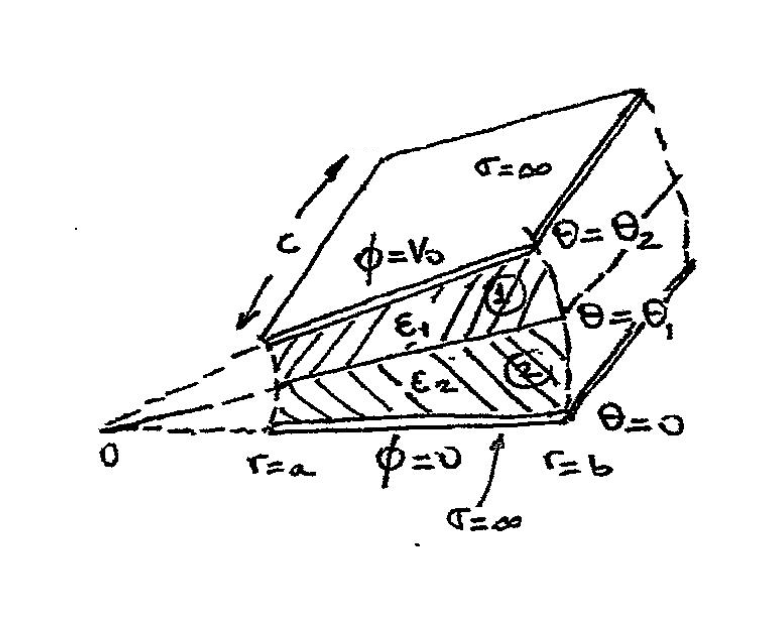
\includegraphics[width=0.7\textwidth]{Control_1_1} % Descomenta y pon el nombre correcto de la imagen
  \caption{A la izquierda se encuentra la posición de equilibrio y la segunda en movimiento del modelo de sistema masa-resorte-amortiguador sobre superficie lunar.}
  \label{fig:modelo_luna}
\end{figure}

\begin{figure}[H]
  \centering
  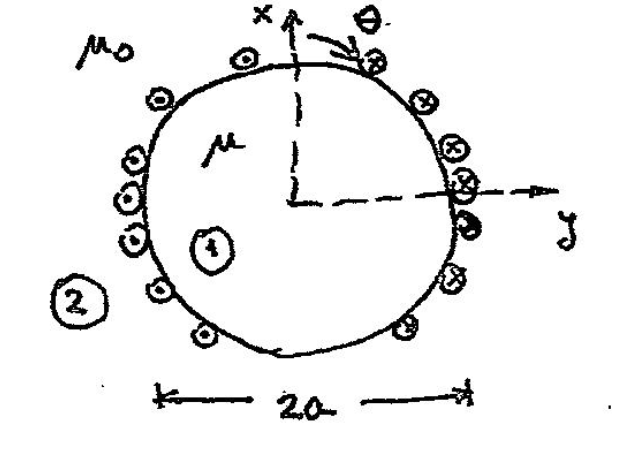
\includegraphics[width=0.5\textwidth]{Control_1_2} % Cambia el nombre si es necesario
  \caption{Perfil de la superficie lunar modelada como función cosenoidal.}
  \label{fig:superficie_lunar}
\end{figure}

\begin{enumerate}
  \item \textbf{[1 punto]} Establezca las hipótesis simplificatorias que sean necesarias. 
  \item \textbf{[2 puntos]} Encuentre la EDO que modela este sistema considerando que el amortiguador es de un tipo especial tal que es proporcional al cuadrado de la velocidad de la masa acoplada.

  \item \textbf{[1.5 puntos]} Reescriba el sistema de forma matricial, además encuentre estados cero, equilibrio y tierra (en caso de existir).

  \item \textbf{[1 punto]} Linealice en torno a un punto de operación arbitrario ($\vec{X}(t), u(t)$). Donde $\vec{X}(t)$ corresponde al vector de estados y $u(t)$ a la variable de entrada.

  \item \textbf{[0.5 puntos]} Del paso anterior, señale el vector de estados, la matriz de estados, la matriz de entrada, la variable de entrada y la variable de salida.

\end{enumerate}

%--------------------------
\begin{solution}
\subsection*{Resolución 1.1}
Las siguientes hipótesis simplificatorias se consideran razonables para el modelo:
\begin{itemize}
  \item La masa $m$ del vehículo es constante y se considera concentrada en un solo punto (modelo de partícula).
  \item El resorte tiene constante elástica $k$ y cumple la ley de Hooke en todo el rango de operación.
  \item El amortiguador tiene una fuerza proporcional al cuadrado de la velocidad, es decir, $F_c = c \dot{x}^2$ (según lo indicado en el enunciado).
  \item El contacto entre la rueda y la superficie lunar es perfecto, es decir, no hay deslizamiento ni pérdidas por fricción adicionales.
  \item La superficie lunar se modela como una función cosenoidal conocida y no cambia con el tiempo.
  \item Se desprecia la resistencia del aire y cualquier otra fuerza externa distinta a las consideradas.
  \item El movimiento se considera unidimensional a lo largo de la dirección $s$.
  \item Los parámetros $m$, $c$, $k$, $a$ y $L$ son constantes y conocidos.
  \item \dots
\end{itemize}

\subsection*{Resolución 1.2}

Para modelar el movimiento del centro de masa $x$ del vehículo respecto al suelo $y$, aplicamos la segunda ley de Newton considerando todas las fuerzas relevantes:
\begin{itemize}
  \item \textbf{Fuerza del resorte:} $-k(x - y)$, donde $x$ es la posición de la masa y $y$ la posición de la superficie lunar bajo la rueda.
  \item \textbf{Fuerza del amortiguador no lineal:} $-c\dot{x}^2$, proporcional al cuadrado de la velocidad.
\end{itemize}

La ecuación de movimiento es:
\begin{align}
  m\ddot{x} &= -k(x - y) - c\dot{x}^2\\
  m\ddot{x} &= -kx + ky - c\dot{x}^2 \\
  m\ddot{x} + c\dot{x}^2 + kx &= ky
\end{align}

Dado que la superficie lunar se modela como
\begin{equation}
  y(t) = a\cos\left(\frac{2\pi s(t)}{L}\right)
\end{equation}
y si el vehículo avanza a velocidad constante $v$, entonces $s(t) = vt$ y por lo tanto:
\begin{equation}
  y(t) = a\cos\left(\frac{2\pi v t}{L}\right)
\end{equation}

Las condiciones iniciales, para generalidad, pueden ser:
\begin{align}
  \dot{x}(0) &= x_0 \\
  x(0) - y(0) &= l_0
\end{align}
Si el vehículo parte en $t=0$ sobre un máximo de la superficie ($y(t=0) =a\cos(0) = a$), entonces:
\begin{align}
  x(0) - a &= l_0 \implies x(0) = l_0 + a
\end{align}

Por lo tanto, la ecuación diferencial final que modela el sistema es:
\begin{equation}
  \boxed{
    \ddot{x}(t) + \frac{c}{m} \dot{x}^2(t) + \frac{k}{m} x(t) = \frac{k}{m} y(t)
  }
\end{equation}
donde $y(t) = a\cos\left(\frac{2\pi v t}{L}\right)$, con condiciones iniciales $x(0) = l_0 + a$ y $\dot{x}(0) = x_0$.

Esta ecuación describe la dinámica del sistema masa-resorte-amortiguador sobre la superficie lunar modelada, considerando la no linealidad del amortiguador y la excitación periódica del terreno.

\subsection*{Resolución 1.3}


Dado que identificamos que el sistema sera no lineal:
\begin{equation}
  \ddot{x}(t) + \frac{c}{m} \dot{x}^2(t) + \frac{k}{m} x(t) = \frac{k}{m} y(t)
\end{equation}
Como la variable que estamos analizando es $\ddot{x}$ luego el vector de estados sera:
\begin{equation}
  \vec{X}(t) = \begin{pmatrix} x(t) \\ \dot{x}(t) \end{pmatrix}
\end{equation}
El sistema se puede escribir como:
\begin{equation}
  \dot{\vec{X}}(t) = \begin{pmatrix} \dot{x}(t) \\ -\frac{c}{m} \dot{x}^2(t) - \frac{k}{m} x(t) + \frac{k}{m} y(t) \end{pmatrix}
\end{equation}
Donde la salida es:
\begin{equation}
  \vec{Y}(t) = \begin{pmatrix} 1 & 0 \\ 0 & 1 \end{pmatrix} \vec{X}(t)
\end{equation}
Luego queremos analizar los diferentes estados, por lo que tenemos lo siguiente:
\begin{itemize}
    \item \textbf{Estado cero:} El estado cero es aquel para el cual, con entrada y condiciones iniciales nulas, la salida es cero:
\begin{equation}
  \vec{X}_0 = \begin{pmatrix} 0 \\ 0 \end{pmatrix}
\end{equation}

\item \textbf{Estado tierra:} El estado tierra es el estado al que el sistema converge para entrada nula y cualquier condición inicial, si existe. En este caso, si el carro no puede bajar más allá del largo natural del resorte (por ejemplo, $l_0$), entonces:
\begin{equation}
  \vec{X}_t = \begin{pmatrix} 0 \\ 0 \end{pmatrix}
\end{equation}
	\item \textbf{Estado de equilibrio:} El estado de equilibrio $\vec{X}_e$ es aquel para el cual $\dot{\vec{X}}(t) = \vec{0}$ con entrada nula. Imponiendo esta condición:
\begin{align}
  \dot{\vec{X}}_e &= \begin{pmatrix} \dot{x}_e \\ -\frac{c}{m} \dot{x}_e^2 - \frac{k}{m} x_e \end{pmatrix} = \begin{pmatrix} 0 \\ 0 \end{pmatrix}
\end{align}
De la primera ecuación, $\dot{x}_e = 0$. De la segunda, $0 = -\frac{k}{m} x_e$ implica $x_e = 0$.
Por lo tanto,
\begin{equation}
  \vec{X}_e = \begin{pmatrix} 0 \\ 0 \end{pmatrix}
\end{equation}
\end{itemize}
Así, los tres estados especiales coinciden en este sistema bajo entrada nula y con las hipótesis dadas.

\subsection*{Resolución 1.4}

Para linealizar el sistema en torno a un punto de operación arbitrario $\left(\vec{X}_p, y_p\right)$, usamos la expansión de Taylor de primer orden:
\begin{align}
  \dot{\vec{X}}(t) &\approx f(\vec{X}_p, y_p) + \left.\frac{\partial f}{\partial \vec{X}}\right|_{\vec{X}_p, y_p} (\vec{X}(t) - \vec{X}_p) + \left.\frac{\partial f}{\partial y}\right|_{\vec{X}_p, y_p} (y(t) - y_p)
\end{align}

Dado el sistema:
\begin{equation}
  \dot{\vec{X}}(t) = \begin{pmatrix} \dot{x}(t) \\ -\frac{c}{m} \dot{x}^2(t) - \frac{k}{m} x(t) + \frac{k}{m} y(t) \end{pmatrix}
\end{equation}

Calculamos las derivadas parciales:
\begin{align}
  \frac{\partial f}{\partial \vec{X}} =
  \begin{pmatrix}
    \frac{\partial \dot{x}(t)}{\partial x(t)} & \frac{\partial \dot{x}(t)}{\partial \dot{x}(t)} \\
    \frac{\partial}{\partial x(t)}\left(-\frac{c}{m} \dot{x}^2(t) - \frac{k}{m} x(t) + \frac{k}{m} y(t)\right) & \frac{\partial}{\partial \dot{x}(t)}\left(-\frac{c}{m} \dot{x}^2(t) - \frac{k}{m} x(t) + \frac{k}{m} y(t)\right)
  \end{pmatrix}
\end{align}

Evaluando en el punto de operación $\left(\vec{X}_p, y_p\right)$:
\begin{align}
  \left.\frac{\partial f}{\partial \vec{X}}\right|_{\vec{X}_p, y_p} =
  \begin{pmatrix}
    0 & 1 \\
    -\frac{k}{m} & -\frac{2c}{m} \dot{x}_p
  \end{pmatrix}
\end{align}

La derivada parcial respecto a $y(t)$ es:
\begin{align}
  \left.\frac{\partial f}{\partial y}\right|_{\vec{X}_p, y_p} = \begin{pmatrix} 0 \\ \frac{k}{m} \end{pmatrix}
\end{align}

Por lo tanto, el sistema linealizado alrededor del punto de operación $\left(\vec{X}_p, y_p\right)$ se expresa como:
\begin{align}
  \dot{\vec{X}}(t) &\approx f(\vec{X}_p, y_p) +
  \begin{pmatrix}
    0 & 1 \\
    -\frac{k}{m} & -\frac{2c}{m} \dot{x}_p
  \end{pmatrix}
  (\vec{X}(t) - \vec{X}_p) +
  \begin{pmatrix} 0 \\ \frac{k}{m} \end{pmatrix} (y(t) - y_p)
\end{align}

\subsection*{Resolución 1.5}
A partir de la linealización realizada, identificamos los siguientes elementos del sistema en espacio de estados:

\begin{itemize}
  \item \textbf{Vector de estados:}
  \begin{equation}
    \vec{X}(t) = \begin{pmatrix} x(t) \\ \dot{x}(t) \end{pmatrix}
  \end{equation}
  \item \textbf{Matriz de estados (evaluada en el punto de operación $\vec{X}_p$):}
  \begin{equation}
    A = \begin{pmatrix} 0 & 1 \\ -\frac{k}{m} & -\frac{2c}{m} \dot{x}_p \end{pmatrix}
  \end{equation}
  \item \textbf{Matriz de entrada:}
  \begin{equation}
    B = \begin{pmatrix} 0 \\ \frac{k}{m} \end{pmatrix}
  \end{equation}
  \item \textbf{Variable de entrada:}
  \begin{equation}
    u(t) = y(t)
  \end{equation}
  \item \textbf{Matriz de salida:}
  \begin{equation}
    C = \begin{pmatrix} 1 & 0 \\ 0 & 1 \end{pmatrix}
  \end{equation}
  \item \textbf{Variable de salida:}
  \begin{equation}
    \vec{Y}(t) = C \vec{X}(t)
  \end{equation}
\end{itemize}

Así, el sistema linealizado queda completamente caracterizado en términos de sus matrices y variables principales.
\end{solution}
%--------------------------

\question
Sea el siguiente sistema en espacio de estados discretos:
\begin{equation}
  \vec{X}[n+1] = \begin{pmatrix} 0 & -1 & 0 \\ 1 & 0 & 0 \\ 0 & 0 & \frac{1}{2} \end{pmatrix} \vec{X}[n] + \begin{pmatrix} 1 \\ 1 \\ 1 \end{pmatrix} u[n]
\end{equation}
\begin{equation}
  y[n] = \begin{pmatrix} 0 & 0 & 1 \end{pmatrix} \vec{X}[n],
\end{equation}
Determine:
\begin{enumerate}
  \item Determine la matriz de transición de estados y funciones base.

  \item Determine la respuesta al impulso del sistema

  \item   Analice la estabilidades BIBO y BIBS del sistema.

  \item Verifique la controlabilidad y observabilidad del sistema.

  \item Mediante retroalimentación de estados ubique los polos en $\{0.2,\;0.3\pm 0.2j\}$.

  \item  Discuta si el control anterior es implementable cuando no se mide el estado
  y el sistema no es completamente observable.
\end{enumerate}
%--------------------------
\begin{solution}
\subsection*{Resolución 2.1}
Se busca obtener la matriz de transición de estados $\Phi[n]$ y las funciones base del sistema. Podemos reconocer que es una matriz de Jordan, por lo tanto:
\begin{equation}
  \vec{X}[n+1] =
  \left(
    \begin{array}{c|c}
      \fbox{$\begin{array}{cc} 0 & -1 \\ 1 & 0 \end{array}$} & \begin{array}{c} 0 \\ 0 \end{array} \\
      \hline
      \begin{array}{cc} 0 & 0 \end{array} & \boxed{\frac{1}{2}}
    \end{array}
  \right)
  \vec{X}[n] + \begin{pmatrix} 1 \\ 1 \\ 1 \end{pmatrix} u[n]
\end{equation}
Lo cual reconocemos por un lado que el primer bloque sera:
\begin{equation}
  \Phi_1[n] = \begin{pmatrix} \cos\left(\frac{\pi}{2} n\right) & -\sin\left(\frac{\pi}{2} n\right) \\ \sin\left(\frac{\pi}{2} n\right) & \cos\left(\frac{\pi}{2} n\right) \end{pmatrix}
\end{equation}
Y el segundo bloque sera:
\begin{equation}
  \Phi_2[n] = \left(\frac{1}{2}\right)^n
\end{equation}
Por lo tanto la matriz de transición de estados sera:
\begin{equation}
  \Phi[n] = \begin{pmatrix} \cos\left(\frac{\pi}{2} n\right) & -\sin\left(\frac{\pi}{2} n\right) & 0 \\ \sin\left(\frac{\pi}{2} n\right) & \cos\left(\frac{\pi}{2} n\right) & 0 \\ 0 & 0 & \left(\frac{1}{2}\right)^n \end{pmatrix}
\end{equation}
Las funciones base las obtenemos mediante la respuesta a entrada cero, es decir:
\begin{align}
  y_{0}[n] = C \Phi[n] \vec{X}[0] &= \begin{pmatrix} 0 & 0 & 1 \end{pmatrix} \begin{pmatrix} \cos\left(\frac{\pi}{2} n\right
) & -\sin\left(\frac{\pi}{2} n\right) & 0 \\ \sin\left(\frac{\pi}{2} n\right) & \cos\left(\frac{\pi}{2} n\right) & 0 \\ 0 & 0 & \left(\frac{1}{2}\right)^n \end{pmatrix} \begin{pmatrix} x_1[0] \\ x_2[0] \\ x_3[0] \end{pmatrix}\\
    &= \begin{pmatrix} 0 & 0 & \left(\frac{1}{2}\right)^n \end{pmatrix} \begin{pmatrix} x_1[0] \\ x_2[0] \\ x_3[0] \end{pmatrix}\\
     &= x_3[0] \left(\frac{1}{2}\right)^n
\end{align}
Con lo que tenemos que la función base es:
\begin{equation}
  h_0[n] = \left(\frac{1}{2}\right)^n
\end{equation}
Otro metodo de Resolución seria el diagonalizar la matriz entera, por lo tanto se tendria que:
\begin{equation}
  A = \begin{pmatrix} 0 & -1 & 0 \\ 1 & 0 & 0 \\ 0 & 0 & \frac{1}{2} \end{pmatrix}
\end{equation}
Calculando los autovalores:
\begin{align}
  \det(A - \lambda I) &= \det\begin{pmatrix} -\lambda & -1 & 0 \\ 1 & -\lambda & 0 \\ 0 & 0 & \frac{1}{2} - \lambda \end{pmatrix}\\
  &= (-\lambda)(-\lambda)(\frac{1}{2} - \lambda) - (-1)(1)(\frac{1}{2} - \lambda)\\
  &= (\lambda^2 + 1)(\frac{1}{2} - \lambda)
\end{align}
Igualando a cero, los autovalores son:
\begin{equation}
  \lambda_1 = j, \quad \lambda_2 = -j, \quad \lambda_3 = \frac{1}{2}
\end{equation}
Calculando los autovectores:
\begin{itemize}
  \item Para $\lambda_1 = j$:
  \begin{align}
    (A - jI)\vec{v}_1 &= 0 \\
    \begin{pmatrix} -j & -1 & 0 \\ 1 & -j & 0 \\ 0 & 0 & \frac{1}{2} - j \end{pmatrix} \begin{pmatrix} v_{11} \\ v_{12} \\ v_{13} \end{pmatrix} &= 0
  \end{align}
  De la tercera fila, $v_{13} = 0$. De las primeras dos filas, obtenemos $v_{12} = -j v_{11}$. Tomando $v_{11} = 1$, entonces:
  \begin{equation}
    \vec{v}_1 = \begin{pmatrix} 1 \\ -j \\ 0 \end{pmatrix}
  \end{equation}

  \item Para $\lambda_2 = -j$:
  \begin{align}
    (A + jI)\vec{v}_2 &= 0 \\
    \begin{pmatrix} j & -1 & 0 \\ 1 & j & 0 \\ 0 & 0 & \frac{1}{2} + j \end{pmatrix} \begin{pmatrix} v_{21} \\ v_{22} \\ v_{23} \end{pmatrix} &= 0
  \end{align}
  De la tercera fila, $v_{23} = 0$. De las primeras dos filas, obtenemos $v_{22} = j v_{21}$. Tomando $v_{21} = 1$, entonces:
  \begin{equation}
    \vec{v}_2 = \begin{pmatrix} 1 \\ j \\ 0 \end{pmatrix}
  \end{equation}

  \item Para $\lambda_3 = \frac{1}{2}$:
  \begin{align}
    (A - \frac{1}{2}I)\vec{v}_3 &= 0 \\
    \begin{pmatrix} -\frac{1}{2} & -1 & 0 \\ 1 & -\frac{1}{2} &
  0 \\ 0 & 0 & 0 \end{pmatrix} \begin{pmatrix} v_{31} \\ v_{32} \\ v_{33} \end{pmatrix} &= 0
  \end{align}
  De la tercera fila, no hay restricción sobre $v_{33}$. De las primeras dos filas, obtenemos $v_{32} = -\frac{1}{2} v_{31}$. Tomando $v_{31} = 1$, entonces:
  \begin{equation}
    \vec{v}_3 = \begin{pmatrix} 1 \\ -\frac{1}{2} \\ 1 \end{pmatrix}
  \end{equation}
\end{itemize}
Formando la matriz de autovectores:
\begin{equation}
  V = \begin{pmatrix} 1 & 1 & 1 \\ -j & j & -\frac{1}{2} \\ 0 & 0 & 1 \end{pmatrix}
\end{equation}
Calculando la inversa de $T$:
\begin{equation}
  V^{-1} = \begin{pmatrix} \frac{1}{2} & \frac{j}{2} & \frac{1}{2} \\ \frac{1}{2} & -\frac{j}{2} & \frac{1}{2} \\ 0 & 0 & 1 \end{pmatrix}
\end{equation}
La matriz diagonal de autovalores es:
\begin{equation}
  D = \begin{pmatrix} j & 0 & 0 \\ 0 & -j & 0 \\ 0 & 0 & \frac{1}{2} \end{pmatrix}
\end{equation}
La matriz de transición de estados se calcula como:
\begin{align}
  \Phi[n] &= T D^n T^{-1} \\
  &= \begin{pmatrix} 1 & 1 & 1 \\ -j & j & -\frac{1}{2} \\ 0 & 0 & 1 \end{pmatrix} \begin{pmatrix} j^n & 0 & 0 \\ 0 & (-j)^n & 0 \\ 0 & 0 & \left(\frac{1}{2}\right)^n \end{pmatrix} \begin{pmatrix} \frac{1}{2} & \frac{j}{2} & \frac{1}{2} \\ \frac{1}{2} & -\frac{j}{2} & \frac{1}{2} \\ 0 & 0 & 1 \end{pmatrix}
\end{align}

Primero multiplicamos $T \cdot D^n$:
\begin{align}
  T D^n &= \begin{pmatrix} 1 & 1 & 1 \\ -j & j & -\frac{1}{2} \\ 0 & 0 & 1 \end{pmatrix} \begin{pmatrix} j^n & 0 & 0 \\ 0 & (-j)^n & 0 \\ 0 & 0 & \left(\frac{1}{2}\right)^n \end{pmatrix} \\
  &= \begin{pmatrix} j^n & (-j)^n & \left(\frac{1}{2}\right)^n \\ -j \cdot j^n & j \cdot (-j)^n & -\frac{1}{2} \cdot \left(\frac{1}{2}\right)^n \\ 0 & 0 & \left(\frac{1}{2}\right)^n \end{pmatrix} \\
  &= \begin{pmatrix} j^n & (-j)^n & \left(\frac{1}{2}\right)^n \\ -j^{n+1} & j(-j)^n & -\frac{1}{2^{n+1}} \\ 0 & 0 & \left(\frac{1}{2}\right)^n \end{pmatrix}
\end{align}

Luego multiplicamos $(T D^n) \cdot T^{-1}$:
\begin{align}
  \Phi[n] &= (T D^n) T^{-1} \\
  &= \begin{pmatrix} j^n & (-j)^n & \left(\frac{1}{2}\right)^n \\ -j^{n+1} & j(-j)^n & -\frac{1}{2^{n+1}} \\ 0 & 0 & \left(\frac{1}{2}\right)^n \end{pmatrix} \begin{pmatrix} \frac{1}{2} & \frac{j}{2} & \frac{1}{2} \\ \frac{1}{2} & -\frac{j}{2} & \frac{1}{2} \\ 0 & 0 & 1 \end{pmatrix}\\
  &= \begin{pmatrix} \frac{1}{2}j^n + \frac{1}{2}(-j)^n & \frac{j}{2}(j^n - (-j)^n) & \frac{1}{2}\left(\frac{1}{2}\right)^n \\ -\frac{1}{2}j^{n+1} + \frac{1}{2^{n+1}} & -\frac{j}{2}j(-j)^n + \frac{1}{2^{n+1}} & -\frac{1}{2^{n+1}} \\ 0 & 0 & \left(\frac{1}{2}\right)^n \end{pmatrix}
\end{align}

Recordando que $j = e^{j\pi/2}$ y $-j = e^{-j\pi/2}$, entonces:
\begin{align}
j^n &= (e^{j\pi/2})^n = e^{jn\pi/2} \\
(-j)^n &= (e^{-j\pi/2})^n = e^{-jn\pi/2}
\end{align}

Usando las fórmulas de Euler: $e^{j\theta} + e^{-j\theta} = 2\cos(\theta)$ y $e^{j\theta} - e^{-j\theta} = 2j\sin(\theta)$:
\begin{align}
j^n + (-j)^n &= e^{jn\pi/2} + e^{-jn\pi/2} = 2\cos\left(\frac{n\pi}{2}\right) \\
j^n - (-j)^n &= e^{jn\pi/2} - e^{-jn\pi/2} = 2j\sin\left(\frac{n\pi}{2}\right)
\end{align}

Calculando el producto, obtenemos:
\begin{equation}
  \Phi[n] = \begin{pmatrix} \cos\left(\frac{\pi}{2} n\right) & -\sin\left(\frac{\pi}{2} n\right) & 0 \\ \sin\left(\frac{\pi}{2} n\right) & \cos\left(\frac{\pi}{2} n\right) & 0 \\ 0 & 0 & \left(\frac{1}{2}\right)^n \end{pmatrix}
\end{equation}

\subsection*{Resolución 2.2}
Se busca determinar la respuesta al impulso, dado que anteriormente obtuvimos la matriz de transición de estados, podemos usar la siguiente ecuación:
\begin{align}
  h[n]&= C\Phi[n] B\\
  &= \begin{pmatrix} 0 & 0 & 1 \end{pmatrix} \begin{pmatrix} \cos\left(\frac{\pi}{2} n\right) & -\sin\left(\frac{\pi}{2} n\right) & 0 \\ \sin\left(\frac{\pi}{2} n\right) & \cos\left(\frac{\pi}{2} n\right) & 0 \\ 0 & 0 & \left(\frac{1}{2}\right)^n \end{pmatrix} \begin{pmatrix} 1 \\ 1 \\ 1 \end{pmatrix}\\
  &= \begin{pmatrix} 0 & 0 & \left(\frac{1}{2}\right)^n \end{pmatrix} \begin{pmatrix} 1 \\ 1 \\ 1 \end{pmatrix}\\
  &= \left(\frac{1}{2}\right)^n
\end{align}
Con lo que se obtiene la respuesta al impulso del sistema.
\subsection*{Resolución 2.3}
Se busca obtener la estabilidad BIBO y BIBS del sistema, por lo tanto:
\begin{itemize}

  \item \textbf{Estabilidad BIBS:} Dado que estamos considerando un sistema discreto, luego para que sea BIBS se debe cumplir que todos los polos del sistema estén dentro del círculo unitario, dado que nuestros polos son:

  \begin{itemize}
    \item El bloque $\begin{pmatrix}0 & 1 \\ -1 & 0\end{pmatrix}$ tiene autovalores $j$ y $-j$ (módulo 1).
    \item El bloque $1/2$ tiene autovalor $1/2$ (módulo $<1$).
  \end{itemize}
  Como hay autovalores en el borde del círculo unitario, el sistema es estable pero no asintóticamente estable. Es decir, para entradas acotadas, el estado no diverge, pero puede oscilar indefinidamente (no decae a cero).

  Por lo tanto, el sistema es BIBS estable, pero no asintóticamente estable, ya que tiene autovalores en el borde del círculo unitario. Si la entrada es acotada, el estado permanece acotado, pero puede haber oscilaciones persistentes.

  \item \textbf{Estabilidad BIBO:} Como la salida depende sólo del tercer estado ($y[n] = [0\ 0\ 1] \vec{X}[n]$), y el modo asociado a $1/2$ es asintóticamente estable, la salida será asintóticamente estable para entradas acotadas. Por lo tanto, el sistema es BIBO estable.
\end{itemize}
\subsection*{Resolución 2.4}
Luego buscamos verificar la controlabilidad y observabilidad del sistema, para ello utilizamos las matrices de controlabilidad y observabilidad para el caso de n=3:
\begin{itemize}
  \item \textbf{Controlabilidad:} La matriz de controlabilidad se define como:
  \begin{equation}
    \mathcal{C} = \begin{pmatrix} B & AB & A^2B \end{pmatrix}
  \end{equation}
  Calculando $AB$ y $A^2B$:
  \begin{align}
    AB &= A \begin{pmatrix} 1 \\ 1 \\ 1 \end{pmatrix} = \begin{pmatrix} -1 \\ 1 \\ \frac{1}{2} \end{pmatrix} \\
    A^2B &= A(AB) = A\begin{pmatrix} -1 \\ 1 \\ \frac{1}{2} \end{pmatrix} = \begin{pmatrix} -1 \\ -1 \\ \frac{1}{4} \end{pmatrix}
  \end{align}
  Por lo tanto, la matriz de controlabilidad es:
  \begin{equation}
    \mathcal{C} = \begin{pmatrix} 1 & -1 & -1 \\ 1 & 1 & -1 \\ 1 & \frac{1}{2} & \frac{1}{4} \end{pmatrix}
  \end{equation}
  Calculando el rango de $\mathcal{C}$:
  \begin{align}
    Rango(\mathcal{C}) &= 3
  \end{align}
  Dado que el rango es igual a la dimensión del estado (3), el sistema es completamente controlable. Tambien se verifica que el determinante de la matriz es diferente de cero, por lo tanto es invertible o viendo que las filas son linealmente independientes.

  \item \textbf{Observabilidad:} La matriz de observabilidad se define como:
  \begin{equation}
    \mathcal{O} = \begin{pmatrix} C \\ CA \\ CA^2 \end{pmatrix}
  \end{equation}
  Calculando $CA$ y $CA^2$:
  \begin{align}
    CA &= C A = \begin{pmatrix} 0 & 0 & 1 \end{pmatrix} A = \begin{pmatrix} 0 & 0 & \frac{1}{2} \end{pmatrix} \\
    CA^2 &= C A^2 = C (AA) = \begin{pmatrix} 0 & 0 & \frac{1}{4} \end{pmatrix}
  \end{align}
  Por lo tanto, la matriz de observabilidad es:
  \begin{equation}
    \mathcal{O} = \begin{pmatrix} 0 & 0 & 1 \\ 0 & 0 & \frac{1}{2} \\ 0 & 0 & \frac{1}{4} \end{pmatrix}
  \end{equation}
  Calculando el rango de $\mathcal{O}$:
  \begin{align}
    Rango(\mathcal{O}) &= 1
  \end{align}
  Dado que el rango es menor que la dimensión del estado (3), el sistema no es completamente observable.
\end{itemize}
Con lo que finalmente tenemos que el sistema es completamente controlable pero no completamente observable.
\subsection*{Resolución 2.5}
Se busca ubicar los polos del sistema en $\{0.2, 0.3 \pm 0.2j\}$ mediante retroalimentación de estados. La ecuación del sistema con retroalimentación de estados es:
\begin{equation}
  \vec{X}[n+1] = (A - BK)\vec{X}[n] + Bu[n]
\end{equation}
Donde $K$ es la ganancia de retroalimentación de estados que queremos determinar. La matriz $A - BK$ debe tener los polos deseados. Primero, calculamos la matriz $A - BK$:
\begin{align}
  A - BK &= \begin{pmatrix} 0 & -1 & 0 \\ 1 & 0 & 0 \\ 0 & 0 & \frac{1}{2} \end{pmatrix} - \begin{pmatrix} 1 \\ 1 \\ 1 \end{pmatrix} \begin{pmatrix} k_1 & k_2 & k_3 \end{pmatrix} \\
  &= \begin{pmatrix} -k_1 & -1 - k_2 & -k_3 \\ 1 - k_1 & -k_2 & -k_3 \\ -k_1 & -k_2 & \frac{1}{2} - k_3 \end{pmatrix}
\end{align}
El polinomio característico de $A - BK$ es:
\begin{align}
  \det(zI - (A - BK)) &= \det\begin{pmatrix} z + k_1 & 1 + k_2 & k_3 \\ -1 + k_1 & z + k_2 & k_3 \\ k_1 & k_2 & z - \frac{1}{2} + k_3 \end{pmatrix}
\end{align}
Calculando el determinante:
\begin{align}
  \det(zI - (A - BK)) &= (z + k_1)\left((z + k_2)(z - \frac{1}{2} + k_3) - k_3 k_2\right) \\
  &\quad - (1 + k_2)\left((-1 + k_1)(z - \frac{1}{2} + k_3) - k_3 k_1\right) \\
  &\quad + k_3\left((-1 + k_1)k_2 - (z + k_2)k_1\right)
\end{align}
Luego tenemos que factorizando se obtiene que:
{\normalsize
\begin{align}
 \begin{split}
 z^3 &+ (k_1 + k_2 - \frac{1}{2})z^2 \\
 &+ (k_1 k_2 + k_1 k_3 + k_2 k_3 - k_1 - \frac{1}{2}k_2 - \frac{1}{2}k_3 + 1)z \\
 &+ (-\frac{1}{2}k_1 k_2 + k_1 k_3 + \frac{1}{2}k_2 k_3 - k_3) = 0
 \end{split}
\end{align}}

Expandiendo y simplificando, obtenemos el polinomio característico en función de $k_1$, $k_2$ y $k_3$. Queremos que este polinomio sea igual al polinomio característico deseado:
\begin{equation}
  (z - 0.2)(z - (0.3 + 0.2j))(z - (0.3 - 0.2j)) = z^3 - 0.8z^2 + 0.17z - 0.02
\end{equation}
Igualando los coeficientes, obtenemos un sistema de ecuaciones para $k_1$, $k_2$ y $k_3$, el cual viene dado por:
\begin{align}
  k_1 + k_2 - \frac{1}{2} &= -0.8 \\
  k_1 k_2 + k_1 k_3 + k_2 k_3 - k_1 - \frac{1}{2}k_2 - \frac{1}{2}k_3 + 1 &= 0.17 \\
  -\frac{1}{2}k_1 k_2 + k_1 k_3 + \frac{1}{2}k_2 k_3 - k_3 &= -0.02
\end{align}
Resolviendo este sistema, encontramos:
\begin{align}
  k_1 &= 0.7 \\
  k_2 &= 0.5 \\
  k_3 &= 0.3
\end{align}
Por lo tanto, la ganancia de retroalimentación de estados que ubica los polos en los valores deseados es:
\begin{equation}
  K = \begin{pmatrix} 0.7 & 0.5 & 0.3 \end{pmatrix}
\end{equation}
\subsection*{Resolución 2.6}
Buscamos el analizar si el control anterior es implementable cuando no se mide el estado y el sistema no es completamente observable. Dado que el sistema no es completamente observable, no podemos reconstruir todos los estados del sistema a partir de la salida medida. En particular, en este caso, sólo se mide el tercer estado ($y[n] = [0\ 0\ 1] \vec{X}[n]$), lo que significa que los dos primeros estados no son observables. 
\end{solution}
\end{questions}
\end{document}